\section{Rahmatul Ridha}
\subsection{Pemahaman Teori}
Kerjakan soal berikut ini, masing-masing bernilai 5 untuk hari pertama. Praktek teori penungjang yang dikerjakan dengan deadline besok jam 4 pagi :
\begin{enumerate}
   \item Apa itu fungsi file csv, jelaskan sejarah dan contohnya.
      \begin{itemize}
         \item Apa itu Fungsi file csv
         Format file csv \textit{Comma Separated Values} yaitu suatu format data pada basis data dimana setiap record yang dapat dipisahkan dengan menggunakan tanda koma (`,’) atau juga bisa dengan menggunakan titik koma (`;’) sebagai tanda pemisah antara datu elemen dengan elemen yang lainnya. Selain bahasa programnya yang sederhana, format ini juga dapat dibuka dengan menggunakan berbagai \textit{text-editor} seperti Notepad, Wordpad, dan MS Excel.
  
          File CSV (nilai berbatas koma) merupakan tipa file khusus yang dapat dibuat atau diedit dengan menggunakan excel. File csv menyimpan informasi yang dapat dipisah oleh koma (,), bukan untuk menyimpan informasi dalam kolom. Saat teks dan angka yang disimpan dalam file csv, dapat memudahkan untuk memindahkannya dari satu program ke program yang lainnya.
  
         \item Sejarah CSV
  
          Nilai yang dipisahkan oleh koma adalah format data yang memberi tanggal lebih awal pada komputer pribadi lebih dari satu dekade: kompiler IBM Fortran (level H extended) di bawah OS / 360 mendukungnya pada tahun 1972. Input / output yang diarahkan oleh daftar ("bentuk bebas") didefinisikan dalam FORTRAN 77, disetujui pada tahun 1978. Input yang diarahkan daftar menggunakan koma atau spasi untuk pembatas, sehingga string karakter yang tidak dikutip tidak dapat mengandung koma atau spasi.
  
         Nama "nilai yang dipisahkan koma" dan singkatan "CSV" digunakan pada tahun 1983. Manual untuk komputer Osborne Executive, yang menggabungkan SuperCalc spreadsheet, mendokumentasikan konvensi kutipan CSV yang memungkinkan string berisi koma yang disematkan, tetapi manual tersebut tidak menentukan konvensi untuk menyematkan tanda kutip dalam string yang dikutip. Daftar nilai yang dipisahkan koma lebih mudah untuk diketik (misalnya ke dalam kartu berlubang) daripada data yang selaras dengan kolom tetap dan cenderung menghasilkan hasil yang salah jika suatu nilai dilubangi satu kolom dari lokasi yang dituju.
  
         Pada 2014 IETF menerbitkan RFC7111 yang menjelaskan aplikasi fragmen URI ke dokumen CSV. RFC7111 menentukan bagaimana rentang baris, kolom, dan sel dapat dipilih dari dokumen CSV menggunakan indeks posisi. Pada 2015 W3C, dalam upaya meningkatkan CSV dengan semantik formal, mempublikasikan draft rekomendasi pertama untuk standar metadata CSV, yang dimulai sebagai rekomendasi pada bulan Desember tahun yang sama.
  
         \item Contohnya
         \lstinputlisting[caption = Contoh penggunaan format CSV., firstline=1, lastline=3]{src/1144124/Chapter4/teori.csv}
      \end{itemize}
   \item Aplikasi-aplikasi apa saja yang bisa menciptakan file csv ?
      \begin{itemize}
         \item Text editor (Notepat, Wordpad, dan lain-lain)
         \item Spreadsheet (Microsoft Excel)
      \end{itemize}
   \item Jelaskan bagaimana cara menulis dan membaca file csv diexcel atau spreadsheet.
      \textbf{Menulis File CSV}
      \begin{enumerate}
	      \item Buat dokumen baru diexcel.
         \item Tambahkan judul kolom untuk setiap potongan informasi yang ingin dicatat, contohnya npm, nama, kelas. Lalu ketikkn informasi delam kolom yang sesuai.
	      \item Setelah selesai dibuat, file excel yang telah dibuat akan terlihat seperti \ref{CSV}
		
		   \begin{figure}[H]	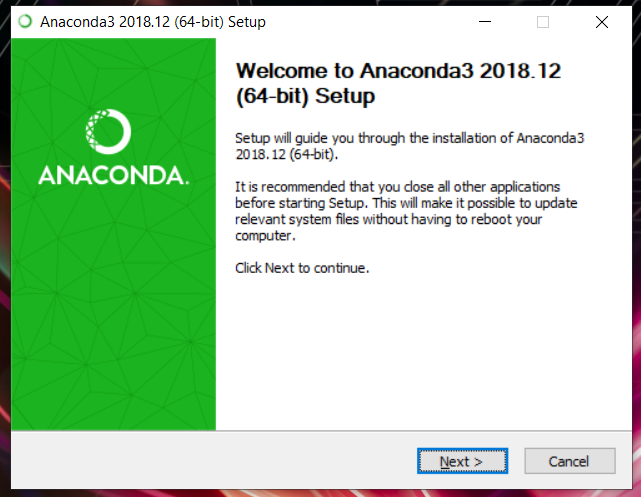
\includegraphics[width=10cm]{figures/rahma/Chapter4/1.png}
		   \centering
         \label{CSV}
		   \end{figure}
		
	      \item Kemudian isi kolom `File name' dengan nama file anda dan kolom `Save as type' pilih yang berekstensi .csv.
		
		   \begin{figure}[H] 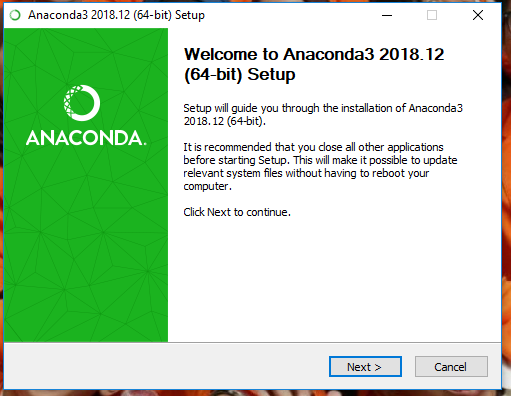
\includegraphics[width=9cm]{figures/rahma/Chapter4/2.png}
			\centering
		   \end{figure}

         \item Kemudian file yang Anda telah terbuat tadi tersimpan dengan ekstensi .csv. Untuk melihat isi filenya tinggal klik dua kali pada file tersebut.
		   \begin{figure}[H]	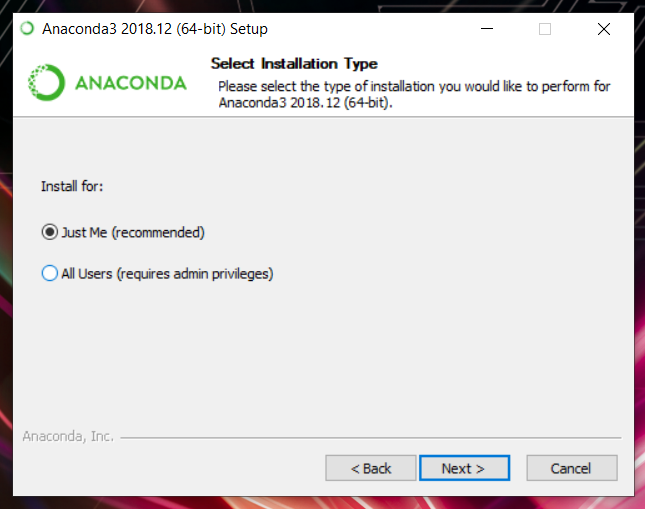
\includegraphics[width=10cm]{figures/rahma/Chapter4/3.png}
			\centering
		   \end{figure}
		
	      \item Lalu tinggal klik `Yes'.	
		   \begin{figure}[H] 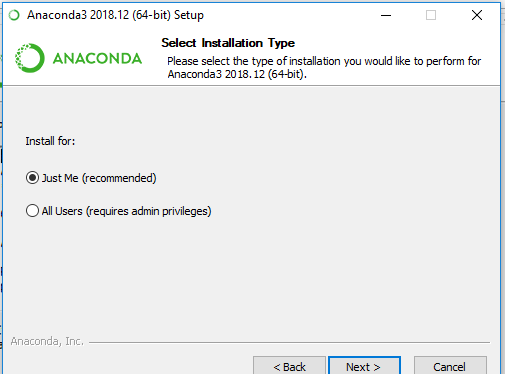
\includegraphics[width=7cm]{figures/rahma/Chapter4/4.png}
			\centering
         \end{figure}
      \end{enumerate}
      \textbf{Melihat File CSV di Excel atau Spreadsheet}
      \begin{enumerate}
        \item Pertama klik dua kali pada file yang yang berekstensi CSV.
        
        \begin{figure}[H]	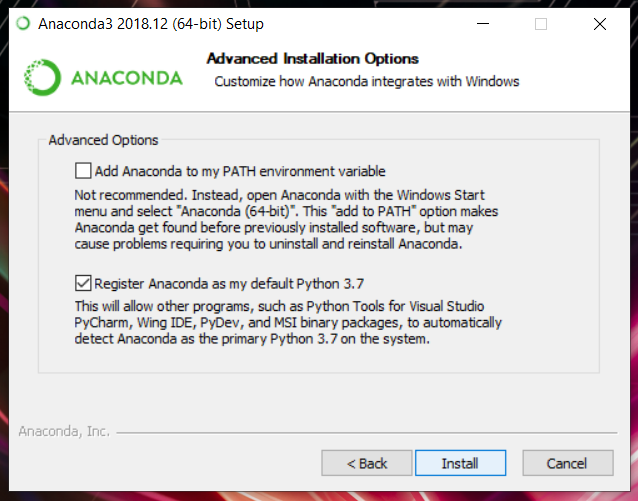
\includegraphics[width=10cm]{figures/rahma/Chapter4/5.png}
           \centering
        \end{figure}
        
        \item Kemudian file akan terbuka secara otomatis di aplikasi Excel atau spreadsheet.
        
        \begin{figure}[H] 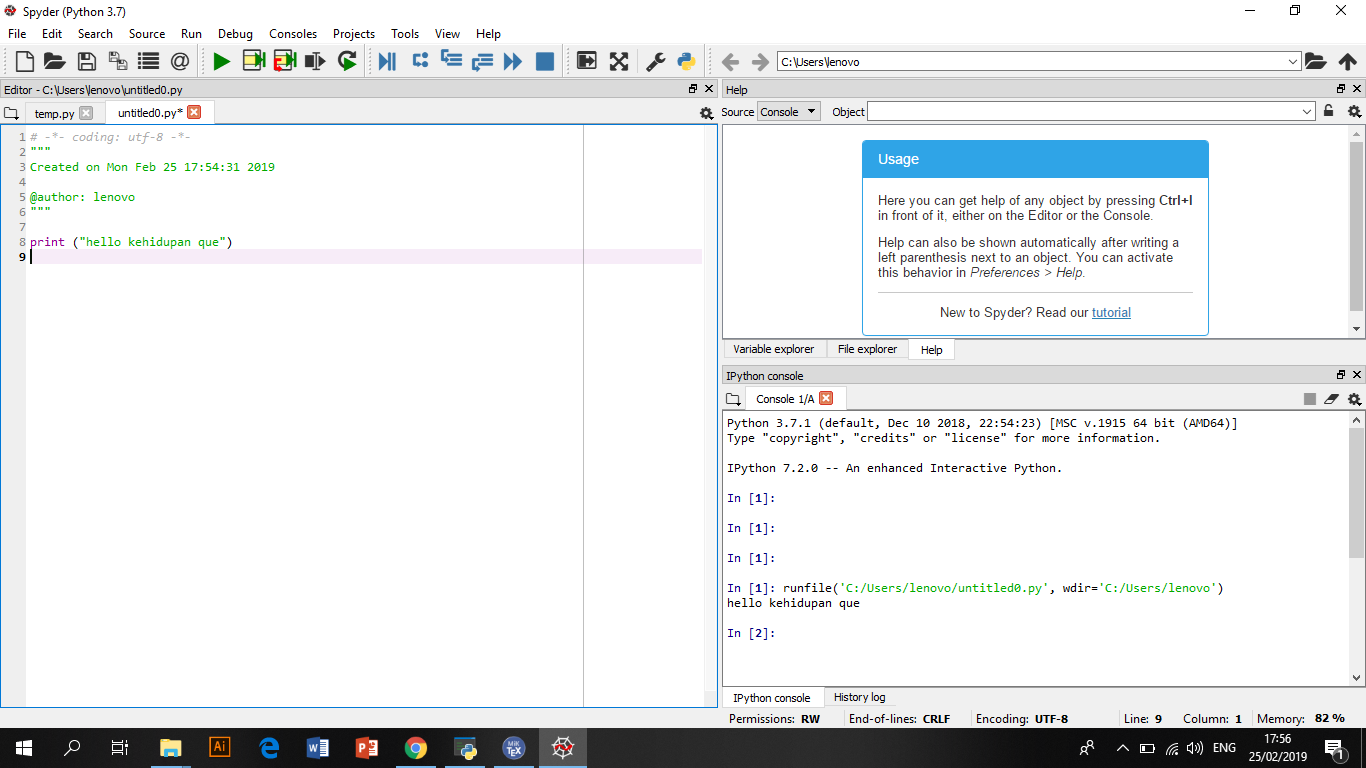
\includegraphics[width=10cm]{figures/rahma/Chapter4/6.png}
           \centering
        \end{figure}
      \end{enumerate}
   \item Jelaskan sejarah library csv.
   Format yang disebut CSV \textit{Comma Separated Values} adalah format impor dan ekspor paling umum untuk spreadsheet dan basis data. Format CSV digunakan selama bertahun-tahun sebelum upaya untuk menggambarkan format dengan cara standar di RFC 4180. Kurangnya standar yang didefinisikan dengan baik berarti bahwa perbedaan halus sering ada dalam data yang diproduksi dan dikonsumsi oleh aplikasi yang berbeda. Perbedaan-perbedaan ini dapat membuatnya menjengkelkan untuk memproses file CSV dari berbagai sumber.
   
   Namun, sementara pembatas dan mengutip karakter bervariasi, format keseluruhan cukup mirip sehingga dimungkinkan untuk menulis satu modul yang dapat secara efisien memanipulasi data seperti itu, menyembunyikan detail membaca dan menulis data dari programmer. Modul csv mengimplementasikan kelas untuk membaca dan menulis data tabular dalam format CSV.
   
   Hal ini memungkinkan programmer untuk mengatakan, "tulis data ini dalam format yang disukai oleh Excel," atau "baca data dari file ini yang dihasilkan oleh Excel," tanpa mengetahui detail yang tepat dari format CSV yang digunakan oleh Excel. Pemrogram juga dapat menggambarkan format CSV yang dipahami oleh aplikasi lain atau menentukan format CSV tujuan khusus mereka sendiri.
   
   \item Jelaskan sejarah library Pandas.
   Pandas merupakan toolkit yang powerfull sebagai alat analisis data dan struktur untuk bahasa pemrograman Python. Dengan menggunakan pandas kita dapat mengolah data dengan mudah, salah satu fiturnya adalah Dataframe. Dengan adanya fitur dataframe kita dapat membaca sebuah file dan menjadikannya tabble, kita juga dapat mengolah suatu data dengan menggunakan operasi seperti join, distinct, group by, agregasi, dan teknik lainnya yang terdapat pada SQL. Banyak format file yang dapat dibaca menggunakan Pandas, seperti file .txt, .csv, .tsv dan lainnya. Agar lebih jelas mari kita mencobanya secara langsung.
   
   \item Jelaskan fungsi-fungsi yang terdapat dilibrary csv.
      \begin{enumerate}
		   \item reader
		
		   Fungsi ini digunakan untuk membaca isi file berformat CSV dari list.
		
		   \lstinputlisting[caption = Membaca file berformat CSV list., firstline=7, lastline=13]{src/1144124/Chapter4/1144124.py}
		
		   \item DictReader
		
		   Fungsi ini digunakan untuk membaca isi file berformat CSV dari dictionary.
		
		   \lstinputlisting[caption =  Membaca file berformat CSV dictionary., firstline=15, lastline=21]{src/1144124/Chapter4/1144124.py}
		
		   \item write
		
		   Fungsi ini digunakan untuk menulis file berformat CSV dari list.
		
		   \lstinputlisting[caption =  Menulis file berformat CSV list., firstline=23, lastline=30]{src/1144124/Chapter4/1144124.py}
		
		   \item DictWrite
		
		   Fungsi ini digunakan untuk menulis file berformat CSV dari dictionary.
		
		   \lstinputlisting[caption =  Menulis file berformat CSV dictionary., firstline=32, lastline=41]{src/1144124/Chapter4/1144124.py}
		
      \end{enumerate}
   \item Jelaskan fungsi-fungsi yang terdapat di library pandas.
      \begin{enumerate}
		   \item read\_csv
		
		   Fungsi ini digunakan untuk membaca isi file berformat CSV
		
		   \lstinputlisting[caption =  Membaca file berformat CSV pandas., firstline=43, lastline=47]{src/1144124/Chapter4/1144124.py}
		
		   \item to\_csv
		
		   Fungsi ini digunakan untuk menulis file berformat CSV
		
		   \lstinputlisting[caption =  Menulis file berformat CSV pandas., firstline=49, lastline=53]{src/1144124/Chapter4/1144124.py}
		
      \end{enumerate}
   \item Cek plagiarisme
   Berikut adalah cek plagiarisme pada teorinya pada \ref{Plagiarisme}
   \begin{figure}[H]
   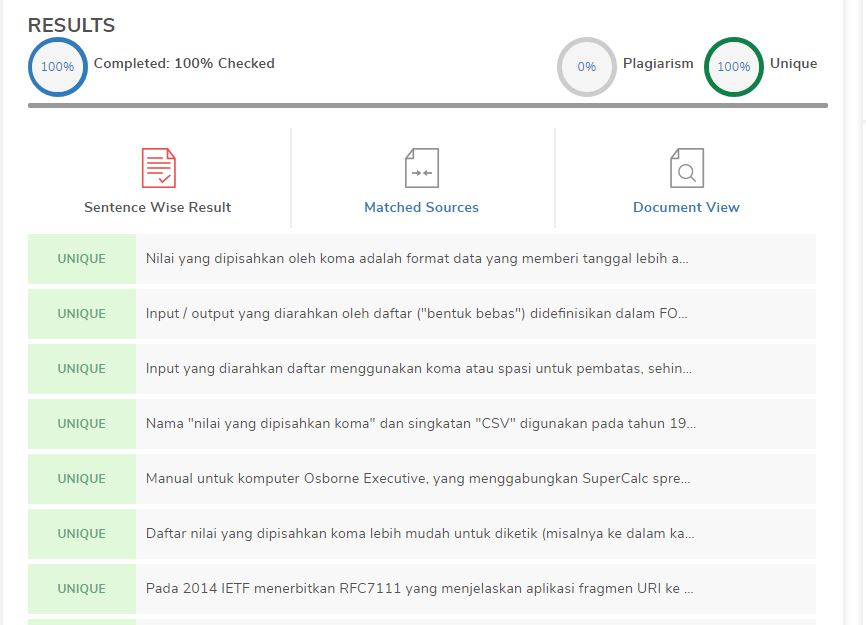
\includegraphics[width=10cm]{figures/rahma/Chapter4/Plagiarisme.jpg}
   \centering
   \label{Plagiarisme}
    \end{figure}
\end{enumerate}
\section{Harun Ar - Rasyid}
 \subsection{Keterampilan Pemograman}
\begin{enumerate}
    \item Buatlah fungsi (file terpisah/library dengan nama NPM csv.py) untuk mem-
    buka file csv dengan lib csv mode list
    Berikut adalah pemanggilan file csv dengan library csv yang menggunakan list
    \lstinputlisting[firstline=10, lastline=20]{src/1174027/c_1174027_csv.py}

    \item Buatlah fungsi (file terpisah/library dengan nama NPM csv.py) untuk mem-
    buka file csv dengan lib csv mode dictionary
    Berikut adalah pemanggilan file csv dengan library csv yang menggunakan dictionary
    \lstinputlisting[firstline=22, lastline=31]{src/1174027/c_1174027_csv.py}

    \item Buatlah fungsi (file terpisah/library dengan nama NPM pandas.py) untuk mem-
    buka file csv dengan lib csv mode list
    Berikut adalah pemanggilan file csv dengan library pandas yang menggunakan list
    \lstinputlisting[firstline=9, lastline=11]{src/1174027/p_1174027_pandas.py}

    \item Buatlah fungsi (file terpisah/library dengan nama NPM pandas.py) untuk mem-
    buka file csv dengan lib csv mode dictionary
    Berikut adalah pemanggilan file csv dengan library pandas yang menggunakan dictionary
    \lstinputlisting[firstline=13, lastline=16]{src/1174027/p_1174027_pandas.py}

    \item Buat fungsi baru di NPM pandas.py untuk mengubah format tanggal menjadi
    standar dataframe
    Berikut penggunaan untuk merubah standar penulisan tanggal, yang mengikuti standar penulisan dari pandas.
    \lstinputlisting[firstline=18, lastline=20]{src/1174027/p_1174027_pandas.py}

    \item Buat fungsi baru di NPM pandas.py untuk mengubah index kolom
    Berikut merupakan pergantian index kolom
    \lstinputlisting[firstline=22, lastline=24]{src/1174027/p_1174027_pandas.py}

    \item Buat fungsi baru di NPM pandas.py untuk mengubah atribut atau nama kolom
    berikut merupakan penggunaan untuk merename atribut yang digunakan, atau merubah nama header 0
    \lstinputlisting[firstline=26, lastline=30]{src/1174027/p_1174027_pandas.py}

    \item Buat program main.py yang menggunakan library NPM csv.py yang membuat
    dan membaca file csv
    \lstinputlisting[firstline=8, lastline=10]{src/1174027/main_harun.py}

    \item Buat program main2.py yang menggunakan library NPM pandas.py yang mem-
    buat dan membaca file csv
    \lstinputlisting[firstline=11, lastline=14]{src/1174027/main_harun.py}
\end{enumerate}


%%%%%%%%%%%%%%%%%%%%%%%%%%%%%%%%%%%%%%%%%%%%%%%%%%%%%%%%%%%%%%%%%%%%%%%%

\section{Kadek Diva Krishna Murti}
\begin{enumerate}
	\item Buatlah  fungsi  (file  terpisah/library  dengan  nama  NPMcsv.py)  untuk  membuka file csv dengan lib csv mode list.
	
	\lstinputlisting[caption = Fungsi untuk membuka file CSV dengan lib CSV mode list., firstline=10, lastline=15]{src/1174006/Chapter4/1174006csv.py}
	
	\item Buatlah  fungsi  (file  terpisah/library  dengan  nama  NPMcsv.py)  untuk  membuka file csv dengan lib csv mode dictionary.
	
	\lstinputlisting[caption =  Fungsi untuk membuka file CSV dengan lib CSV mode dictionary., firstline=17, lastline=22]{src/1174006/Chapter4/1174006csv.py}
	
	\item Buatlah fungsi (file terpisah/library dengan nama NPMpandas.py) untuk membuka file csv dengan lib pandas mode list.
	
	\lstinputlisting[caption =  Fungsi untuk membuka file CSV dengan lib Pandas mode list., firstline=10, lastline=13]{src/1174006/Chapter4/1174006pandas.py}
	
	\item Buatlah fungsi (file terpisah/library dengan nama NPMpandas.py) untuk membuka file csv dengan lib pandas mode dictionary.
	
	\lstinputlisting[caption =  Fungsi untuk membuka file CSV dengan lib Pandas mode dictionary., firstline=10, lastline=13]{src/1174006/Chapter4/1174006pandas.py}
	
	\item  Buat fungsi baru di NPMpandas.py untuk mengubah format tanggal menjadi standar dataframe.
	
	\lstinputlisting[caption =  Fungsi untuk mengubah format tanggal menjadi standar dataframe., firstline=15, lastline=19]{src/1174006/Chapter4/1174006pandas.py}
	
	\item Buat fungsi baru di NPMpandas.py untuk mengubah index kolom.
	
	\lstinputlisting[caption =  Fungsi untuk mengubah index kolom., firstline=21, lastline=24]{src/1174006/Chapter4/1174006pandas.py}
	
	\item Buat fungsi baru di NPMpandas.py untuk mengubah atribut atau nama kolom.
	
	\lstinputlisting[caption =  Fungsi untuk mengubah atribut atau nama kolom., firstline=26, lastline=30]{src/1174006/Chapter4/1174006pandas.py}
	
	\item Buat program main.py yang menggunakan library NPMcsv.py yang membuat dan membaca file csv.
	
	\lstinputlisting[caption =  Membuat dan mebaca file CSV menggunakan library 1174006pandas., firstline=8, lastline=13]{src/1174006/Chapter4/main.py}
	
	\item Buat program main2.py yang menggunakan library NPMpandas.py yang membuat dan membaca file csv.
	
	\lstinputlisting[caption = Membuat dan mmebaca file CSV menggunakan library 1174006pandas., firstline=8, lastline=13]{src/1174006/Chapter4/main2.py}
	
\end{enumerate}

\textbf{Kode Program}
\begin{figure}[H]
	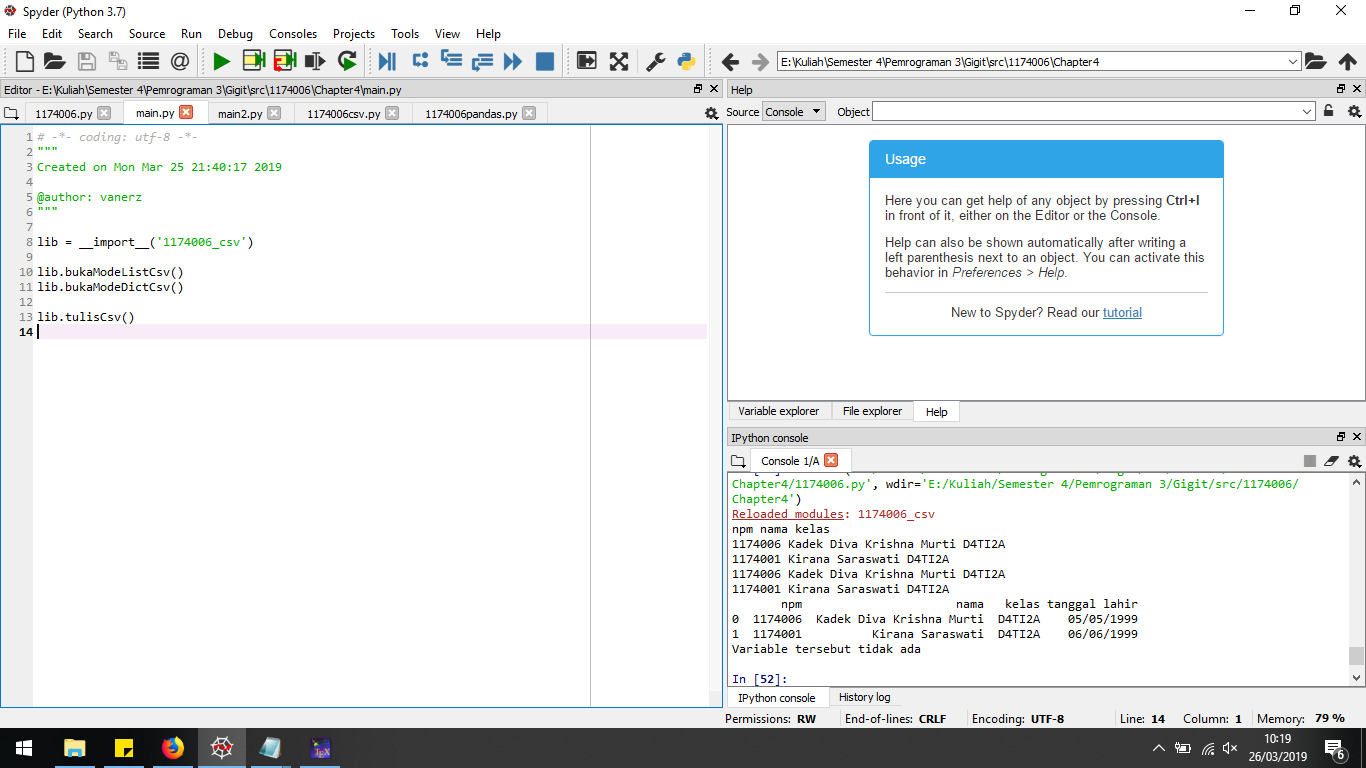
\includegraphics[width=10cm]{figures/diva/Chapter4/harikedua/k1.png}
	\centering
\end{figure}
\begin{figure}[H]
	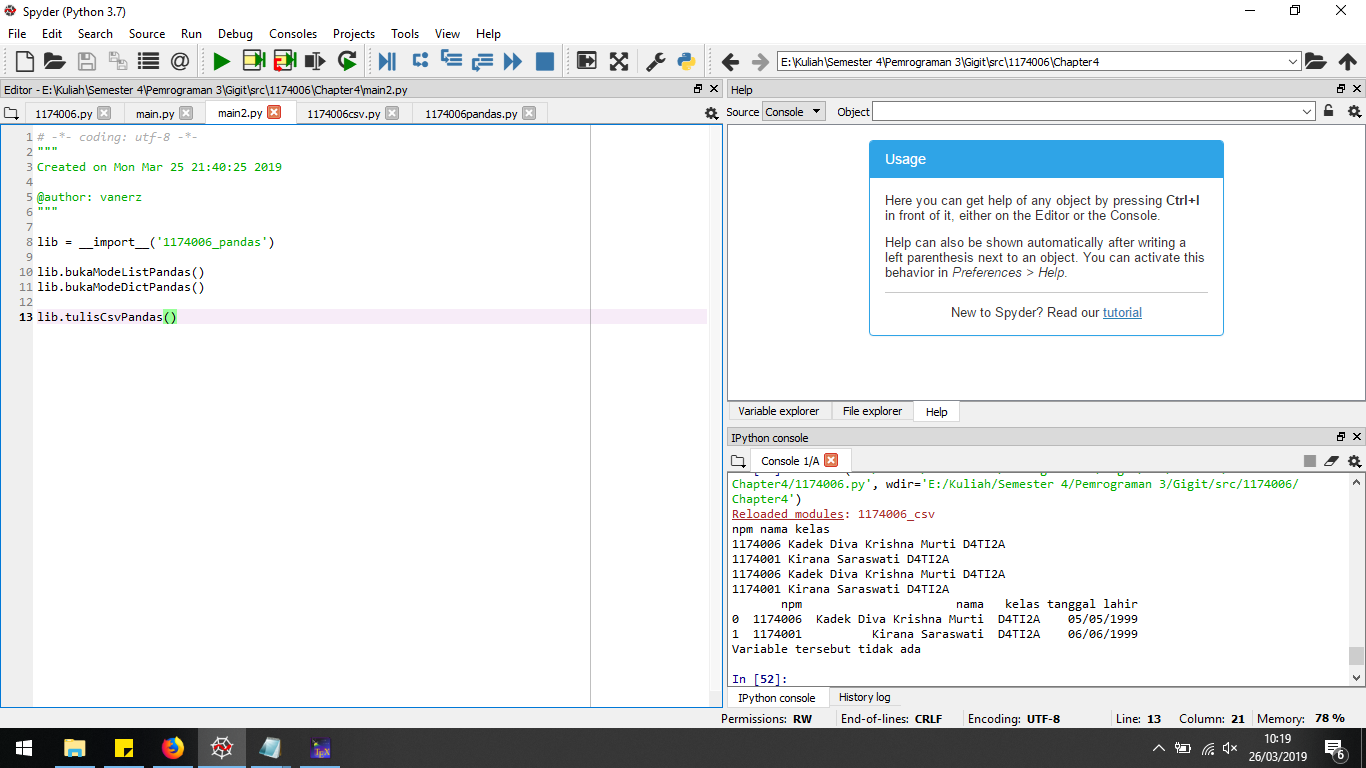
\includegraphics[width=10cm]{figures/diva/Chapter4/harikedua/k2.png}
	\centering
\end{figure}
\begin{figure}[H]
	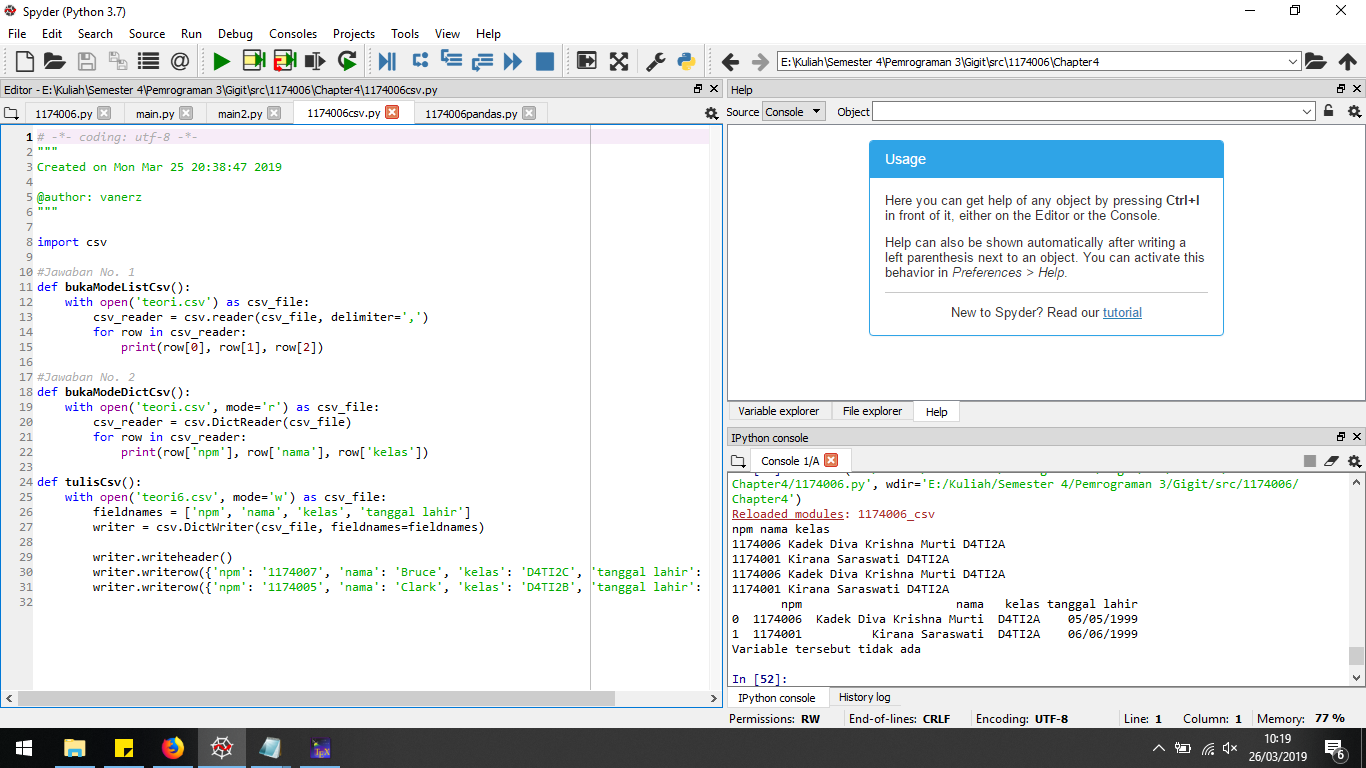
\includegraphics[width=10cm]{figures/diva/Chapter4/harikedua/k3.png}
	\centering
\end{figure}
\begin{figure}[H]
	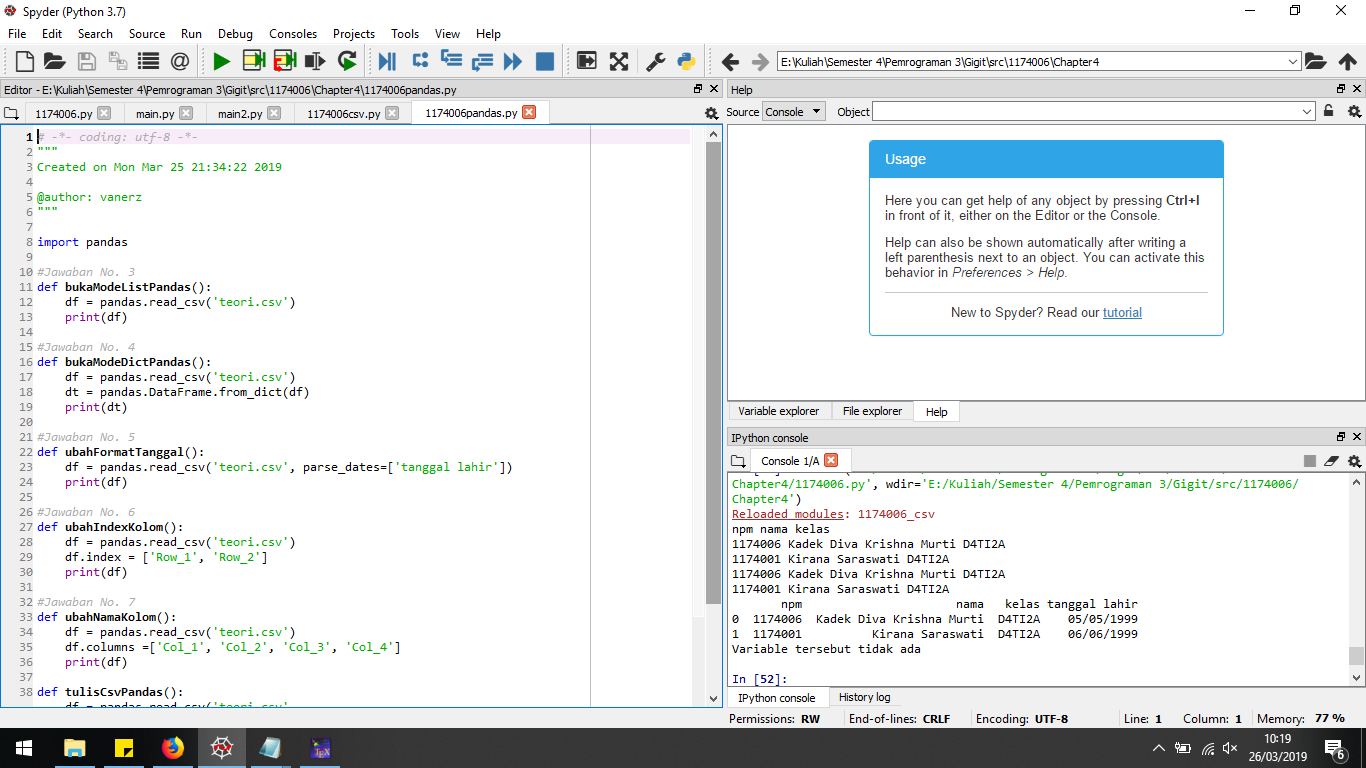
\includegraphics[width=10cm]{figures/diva/Chapter4/harikedua/k4.png}
	\centering
\end{figure}
\begin{figure}[H]
	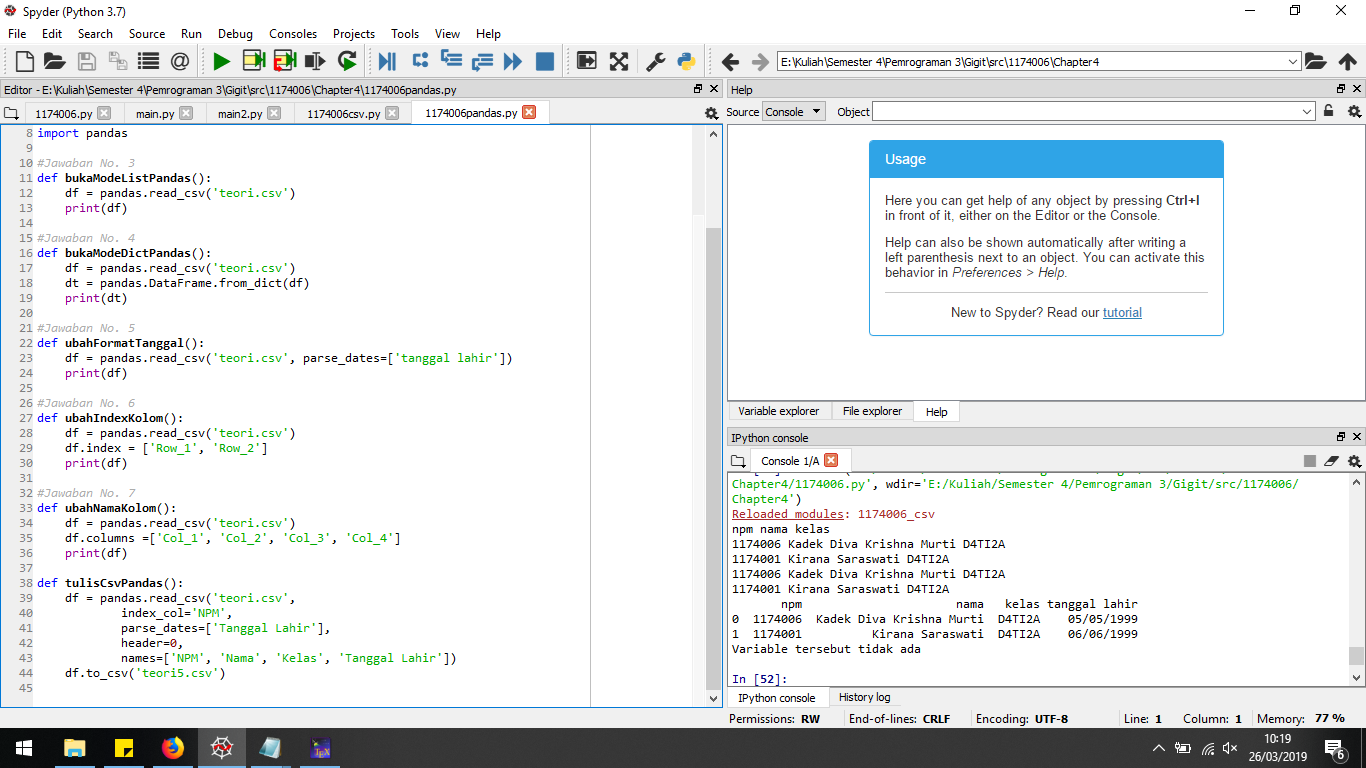
\includegraphics[width=10cm]{figures/diva/Chapter4/harikedua/k5.png}
	\centering
\end{figure}

\textbf{Cek Plagiat}
\begin{figure}[H]
	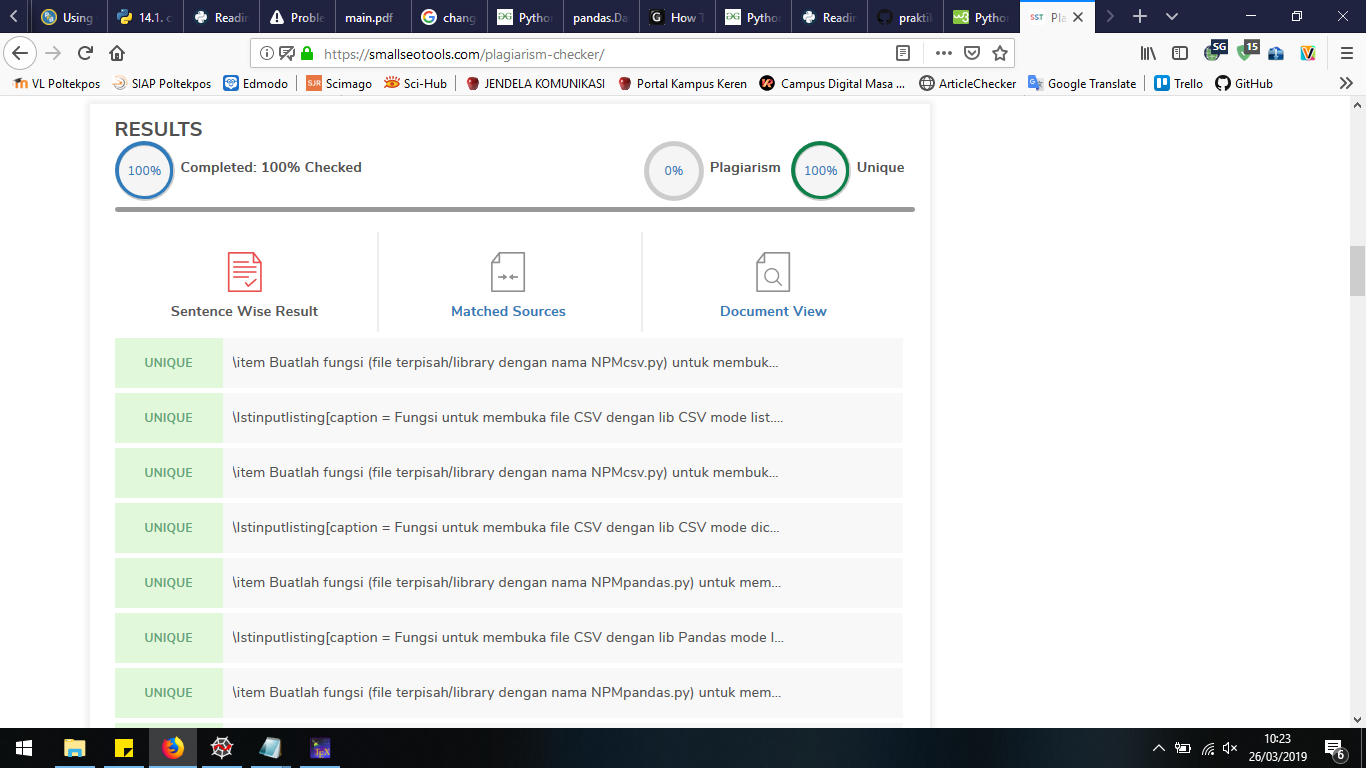
\includegraphics[width=10cm]{figures/diva/Chapter4/harikedua/plagiatketrampilan.png}
	\centering
\end{figure}

%%%%%%%%%%%%%%%%%%%%%%%%%%%%%%%%%%%%%%%%%%%%%%%%%%%%%%%%%%%%%%%%%%%%%%

\section{Dwi Yulianingsih}
\subsection{Praktek}
\begin{enumerate}

\item Buatlah fungsi (file terpisah/library dengan nama NPM csv.py) untuk membuka file csv dengan lib csv mode list
\lstinputlisting[firstline=10, lastline=20]{src/1174009/praktek/d1174009_csv.py}

\item Buatlah fungsi (file terpisah/library dengan nama NPM csv.py) untuk membuka file csv dengan lib csv mode dictionary
\lstinputlisting[firstline=22,lastline=34]{src/1174009/praktek/d1174009_csv.py}

\item Buatlah fungsi (file terpisah/library dengan nama NPM pandas.py) untuk membuka file csv dengan lib pandas mode list
\lstinputlisting[firstline=7,lastline=10]{src/1174009/praktek/d1174009_pandas.py}

\item Buatlah fungsi (file terpisah/library dengan nama NPM pandas.py) untuk membuka file csv dengan lib pandas mode dictionary
\lstinputlisting[firstline=12,lastline=15]{src/1174009/praktek/d1174009_pandas.py}

\item Buat fungsi baru di NPM pandas.py untuk mengubah format tanggal menjadi standar dataframe
\lstinputlisting[firstline=17,lastline=19]{src/1174009/praktek/d1174009_pandas.py}

\item Buat fungsi baru di NPM pandas.py untuk mengubah index kolom
\lstinputlisting[firstline=21,lastline=23]{src/1174009/praktek/d1174009_pandas.py}

\item Buat fungsi baru di NPM pandas.py untuk mengubah atribut atau nama kolom
\lstinputlisting[firstline=25,lastline=29]{src/1174009/praktek/d1174009_pandas.py}

\item Buat program main.py yang menggunakan library NPM csv.py yang membuat dan membaca file csv
\lstinputlisting[firstline=8,lastline=10]{src/1174009/praktek/main_dwi.py}

\item Buat program main2.py yang menggunakan library NPM pandas.py yang membuat dan membaca file csv
\lstinputlisting[firstline=12,lastline=14]{src/1174009/praktek/main_dwi.py}

\end{enumerate}